\documentclass{article}
\usepackage[T1]{fontenc}
\usepackage{iclr2026_conference,times}
\input{math_commands.tex}
\usepackage{hyperref}
\usepackage{url}
\usepackage{amsmath,amssymb}
\usepackage{graphicx}
\usepackage{booktabs}
\usepackage{multirow}
\usepackage{xcolor}
\usepackage{etoolbox}
\graphicspath{{../../}}
\newcommand{\sca}{SCA}
\newcommand{\Oloc}{O^{\mathrm{loc}}}
\newcommand{\Oglob}{O^{\mathrm{glob}}}
\newcommand{\Ofull}{O^{\mathrm{full}}}
\newcommand{\pih}{\pi_{h}(\sigma)}
\begin{document}
\noindent\texttt{snippet: ablation}\par% Generated by paper/figures/src/fig_qual.py ablation; do not edit by hand.
% 1139740195494332405 (4096x4096): A woman with short hair and a black dress stands in a forest, holding an owl with large, outstretched wings. The sunlight filters through the trees, h
% 1516768667427572324 (4096x4096): A cluttered artist's corner features an ornate gold frame, a painting of a man with glasses, several empty picture frames, a vintage suitcase, and var
% 4525259556400020626 (4096x4096): Snow-covered landscape featuring a group of sheep in the foreground, with a quaint, snow-dusted church and rustic houses in the background surrounded 
% 7009273464006889449 (4096x4096): A smiling man in a blue jacket holds a sign labeled "Fantasyland" in front of a stone castle with turrets and flags under a clear sky.
\input{figures/snippets/_scagrid}%
\begin{figure*}[t]
\begingroup\scaGridStyle
\setlength{\scaT}{\dimexpr(\linewidth-20pt-\scaLW-\scaLG)*1000/6000\relax}%
\makebox[\linewidth][c]{\hspace*{\dimexpr\scaLW+\scaLG\relax}\scaHead{\scaT}{scaMid}{No gate}\hspace{4pt}\scaHead{\scaT}{scaMid}{\scaTwo{$\pi{=}1$}{local only}}\hspace{4pt}\scaHead{\scaT}{scaMid}{Uniform $\pi(\sigma)$}\hspace{4pt}\scaHead{\scaT}{scaMid}{\scaTwo{$\pi{=}0$}{global only}}\hspace{4pt}\scaHead{\scaT}{scaMid}{Mean pooling}\hspace{4pt}\scaHead{\scaT}{scaAccent}{\textcolor{scaAccent}{\textbf{SCA (ours)}}}}\par\vskip2pt
\makebox[\linewidth][c]{\scaRowLabel{\scaT}{Full image}\hspace{\scaLG}\scaFull{\scaT}{\scaT}{figures/ablation/1139740195494332405_abl_v0.jpg}{(0.49414,0.56641)}{(0.61914,0.69141)}\hspace{4pt}\scaFull{\scaT}{\scaT}{figures/ablation/1139740195494332405_abl_local.jpg}{(0.49414,0.56641)}{(0.61914,0.69141)}\hspace{4pt}\scaFull{\scaT}{\scaT}{figures/ablation/1139740195494332405_abl_uniform.jpg}{(0.49414,0.56641)}{(0.61914,0.69141)}\hspace{4pt}\scaFull{\scaT}{\scaT}{figures/ablation/1139740195494332405_abl_global.jpg}{(0.49414,0.56641)}{(0.61914,0.69141)}\hspace{4pt}\scaFull{\scaT}{\scaT}{figures/ablation/1139740195494332405_abl_mean.jpg}{(0.49414,0.56641)}{(0.61914,0.69141)}\hspace{4pt}\scaFull{\scaT}{\scaT}{figures/ablation/1139740195494332405_sca.jpg}{(0.49414,0.56641)}{(0.61914,0.69141)}}\par\vskip1pt
\makebox[\linewidth][c]{\scaRowLabel{\scaT}{1:1 crop}\hspace{\scaLG}\scaCrop{\scaT}{\scaT}{figures/ablation/1139740195494332405_abl_v0_crop.jpg}\hspace{4pt}\scaCrop{\scaT}{\scaT}{figures/ablation/1139740195494332405_abl_local_crop.jpg}\hspace{4pt}\scaCrop{\scaT}{\scaT}{figures/ablation/1139740195494332405_abl_uniform_crop.jpg}\hspace{4pt}\scaCrop{\scaT}{\scaT}{figures/ablation/1139740195494332405_abl_global_crop.jpg}\hspace{4pt}\scaCrop{\scaT}{\scaT}{figures/ablation/1139740195494332405_abl_mean_crop.jpg}\hspace{4pt}\scaCrop{\scaT}{\scaT}{figures/ablation/1139740195494332405_sca_crop.jpg}}\par\vskip5pt
\makebox[\linewidth][c]{\scaRowLabel{\scaT}{Full image}\hspace{\scaLG}\scaFull{\scaT}{\scaT}{figures/ablation/1516768667427572324_abl_v0.jpg}{(0.78711,0.22266)}{(0.91211,0.34766)}\hspace{4pt}\scaFull{\scaT}{\scaT}{figures/ablation/1516768667427572324_abl_local.jpg}{(0.78711,0.22266)}{(0.91211,0.34766)}\hspace{4pt}\scaFull{\scaT}{\scaT}{figures/ablation/1516768667427572324_abl_uniform.jpg}{(0.78711,0.22266)}{(0.91211,0.34766)}\hspace{4pt}\scaFull{\scaT}{\scaT}{figures/ablation/1516768667427572324_abl_global.jpg}{(0.78711,0.22266)}{(0.91211,0.34766)}\hspace{4pt}\scaFull{\scaT}{\scaT}{figures/ablation/1516768667427572324_abl_mean.jpg}{(0.78711,0.22266)}{(0.91211,0.34766)}\hspace{4pt}\scaFull{\scaT}{\scaT}{figures/ablation/1516768667427572324_sca.jpg}{(0.78711,0.22266)}{(0.91211,0.34766)}}\par\vskip1pt
\makebox[\linewidth][c]{\scaRowLabel{\scaT}{1:1 crop}\hspace{\scaLG}\scaCrop{\scaT}{\scaT}{figures/ablation/1516768667427572324_abl_v0_crop.jpg}\hspace{4pt}\scaCrop{\scaT}{\scaT}{figures/ablation/1516768667427572324_abl_local_crop.jpg}\hspace{4pt}\scaCrop{\scaT}{\scaT}{figures/ablation/1516768667427572324_abl_uniform_crop.jpg}\hspace{4pt}\scaCrop{\scaT}{\scaT}{figures/ablation/1516768667427572324_abl_global_crop.jpg}\hspace{4pt}\scaCrop{\scaT}{\scaT}{figures/ablation/1516768667427572324_abl_mean_crop.jpg}\hspace{4pt}\scaCrop{\scaT}{\scaT}{figures/ablation/1516768667427572324_sca_crop.jpg}}\par\vskip5pt
\makebox[\linewidth][c]{\scaRowLabel{\scaT}{Full image}\hspace{\scaLG}\scaFull{\scaT}{\scaT}{figures/ablation/4525259556400020626_abl_v0.jpg}{(0.23047,0.41016)}{(0.35547,0.53516)}\hspace{4pt}\scaFull{\scaT}{\scaT}{figures/ablation/4525259556400020626_abl_local.jpg}{(0.23047,0.41016)}{(0.35547,0.53516)}\hspace{4pt}\scaFull{\scaT}{\scaT}{figures/ablation/4525259556400020626_abl_uniform.jpg}{(0.23047,0.41016)}{(0.35547,0.53516)}\hspace{4pt}\scaFull{\scaT}{\scaT}{figures/ablation/4525259556400020626_abl_global.jpg}{(0.23047,0.41016)}{(0.35547,0.53516)}\hspace{4pt}\scaFull{\scaT}{\scaT}{figures/ablation/4525259556400020626_abl_mean.jpg}{(0.23047,0.41016)}{(0.35547,0.53516)}\hspace{4pt}\scaFull{\scaT}{\scaT}{figures/ablation/4525259556400020626_sca.jpg}{(0.23047,0.41016)}{(0.35547,0.53516)}}\par\vskip1pt
\makebox[\linewidth][c]{\scaRowLabel{\scaT}{1:1 crop}\hspace{\scaLG}\scaCrop{\scaT}{\scaT}{figures/ablation/4525259556400020626_abl_v0_crop.jpg}\hspace{4pt}\scaCrop{\scaT}{\scaT}{figures/ablation/4525259556400020626_abl_local_crop.jpg}\hspace{4pt}\scaCrop{\scaT}{\scaT}{figures/ablation/4525259556400020626_abl_uniform_crop.jpg}\hspace{4pt}\scaCrop{\scaT}{\scaT}{figures/ablation/4525259556400020626_abl_global_crop.jpg}\hspace{4pt}\scaCrop{\scaT}{\scaT}{figures/ablation/4525259556400020626_abl_mean_crop.jpg}\hspace{4pt}\scaCrop{\scaT}{\scaT}{figures/ablation/4525259556400020626_sca_crop.jpg}}\par\vskip5pt
\makebox[\linewidth][c]{\scaRowLabel{\scaT}{Full image}\hspace{\scaLG}\scaFull{\scaT}{\scaT}{figures/ablation/7009273464006889449_abl_v0.jpg}{(0.48438,0.21875)}{(0.60938,0.34375)}\hspace{4pt}\scaFull{\scaT}{\scaT}{figures/ablation/7009273464006889449_abl_local.jpg}{(0.48438,0.21875)}{(0.60938,0.34375)}\hspace{4pt}\scaFull{\scaT}{\scaT}{figures/ablation/7009273464006889449_abl_uniform.jpg}{(0.48438,0.21875)}{(0.60938,0.34375)}\hspace{4pt}\scaFull{\scaT}{\scaT}{figures/ablation/7009273464006889449_abl_global.jpg}{(0.48438,0.21875)}{(0.60938,0.34375)}\hspace{4pt}\scaFull{\scaT}{\scaT}{figures/ablation/7009273464006889449_abl_mean.jpg}{(0.48438,0.21875)}{(0.60938,0.34375)}\hspace{4pt}\scaFull{\scaT}{\scaT}{figures/ablation/7009273464006889449_sca.jpg}{(0.48438,0.21875)}{(0.60938,0.34375)}}\par\vskip1pt
\makebox[\linewidth][c]{\scaRowLabel{\scaT}{1:1 crop}\hspace{\scaLG}\scaCrop{\scaT}{\scaT}{figures/ablation/7009273464006889449_abl_v0_crop.jpg}\hspace{4pt}\scaCrop{\scaT}{\scaT}{figures/ablation/7009273464006889449_abl_local_crop.jpg}\hspace{4pt}\scaCrop{\scaT}{\scaT}{figures/ablation/7009273464006889449_abl_uniform_crop.jpg}\hspace{4pt}\scaCrop{\scaT}{\scaT}{figures/ablation/7009273464006889449_abl_global_crop.jpg}\hspace{4pt}\scaCrop{\scaT}{\scaT}{figures/ablation/7009273464006889449_abl_mean_crop.jpg}\hspace{4pt}\scaCrop{\scaT}{\scaT}{figures/ablation/7009273464006889449_sca_crop.jpg}}\par
\endgroup
\caption{\textbf{Without the gate the subject repeats; $\pi=0$ leaves the pooled branch's coarse grid, and mean pooling loses the layout.} Four ablation prompts at 4096$\times$4096, seed~0, 28 steps, guidance 4.5; variants as in Table~\ref{tab:ablation}; crops show native pixels of the outlined 512$\times$512 windows. $\pi=1$ and uniform $\pi(\sigma)$ look close to SCA here; their deficits show in the metrics.}
\label{fig:ablation_grid}
\end{figure*}

\clearpage
\noindent\texttt{snippet: calib}\par% Generated by paper/figures/src/fig_calib.py; numbers in the caption are printed by that script.
\begin{figure*}[t]
  \centering
  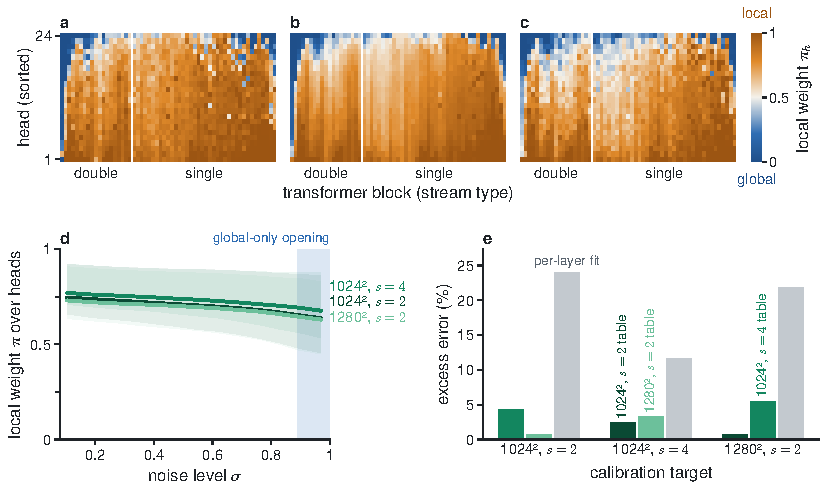
\includegraphics[width=\linewidth]{figures/calib.pdf}
  \caption{\textbf{Heads differ widely, yet a calibrated table transfers across scale and resolution.}
  (a to c) $\pih$ of the scale-4 table used at inference, heads sorted within each block.
  (d) Mean and interquartile range over all 1368 heads for three calibrations (32 prompts at $1024^2$, 16 at $1280^2$).
  (e) Error added over the target's own per-head table: at most 5.45\% for a transferred table, 12 to 24\% for the target's own per-layer fit.}
  \label{fig:calib}
\end{figure*}

\clearpage
\noindent\texttt{snippet: failures}\par% Generated by paper/figures/src/fig_qual.py failures; do not edit by hand.
% 7354534197758042049 (4096x4096): A woman kneels on the forest floor, smiling as she offers grapes to a large brown bear beside her, surrounded by tall birch trees.
% 3614061571823823193 (4096x4096): A Moai statue gazes upward against a starry night sky, with a colorful sunset illuminating the horizon.
% 7396058529551312081 (4096x4096): A woman in a red traditional outfit holds a sword, poised in a dynamic stance, with an intense expression, set against a dark background.
% 1316997283360365550 (4096x4096): A man with a beard stands confidently beside large green and black train wheels, wearing a beige coat over a navy puffer jacket and gray trousers, wit
% m8648158440845565467 (4096x4096): A ballerina in a flowing yellow dress performs an elegant pose on one leg, showcasing her strength and grace against a backdrop of geometric wall art 
% m702025498990232048 (4096x4096): A woman with glasses and a sword poses confidently beside a muscular man in traditional attire holding a sword, while a small creature with a large ha
\begin{figure*}[t]
\centering\sffamily\scriptsize\ifdefined\scaW\else\newlength{\scaW}\fi\setlength{\scaW}{\textwidth}
\setlength{\fboxsep}{1pt}\setlength{\lineskip}{0pt}\setlength{\lineskiplimit}{0pt}
\makebox[\textwidth][l]{\makebox[0.1632\scaW][c]{No gate, window 64}\hspace{0.0040\scaW}\makebox[0.1632\scaW][c]{No gate, window 16}\hspace{0.0040\scaW}\makebox[0.1632\scaW][c]{\textbf{SCA (ours)}}\hspace{0.0040\scaW}\makebox[0.1632\scaW][c]{No gate, window 64}\hspace{0.0040\scaW}\makebox[0.1632\scaW][c]{No gate, window 16}\hspace{0.0040\scaW}\makebox[0.1632\scaW][c]{\textbf{SCA (ours)}}}\\[0.0040\textwidth]
\makebox[\textwidth][l]{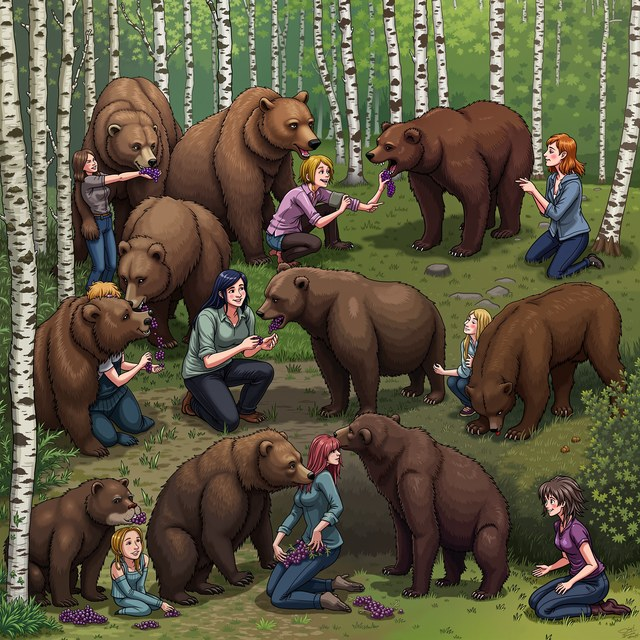
\includegraphics[height=0.1632\scaW]{figures/failures/dup_7354534197758042049_abl_v0.jpg}\hspace{0.0040\scaW}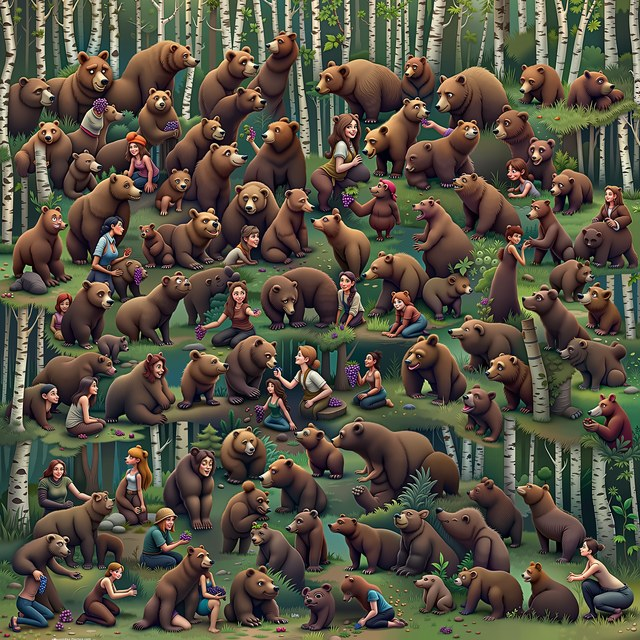
\includegraphics[height=0.1632\scaW]{figures/failures/dup_7354534197758042049_dev_w16.jpg}\hspace{0.0040\scaW}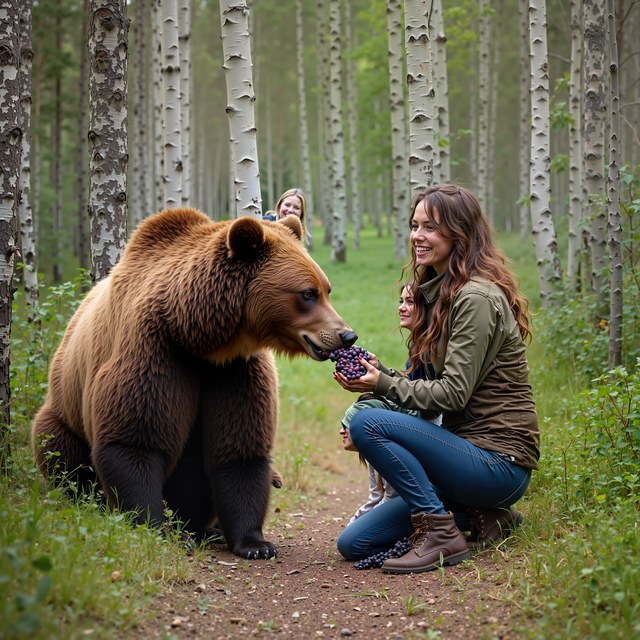
\includegraphics[height=0.1632\scaW]{figures/failures/dup_7354534197758042049_sca.jpg}\hspace{0.0040\scaW}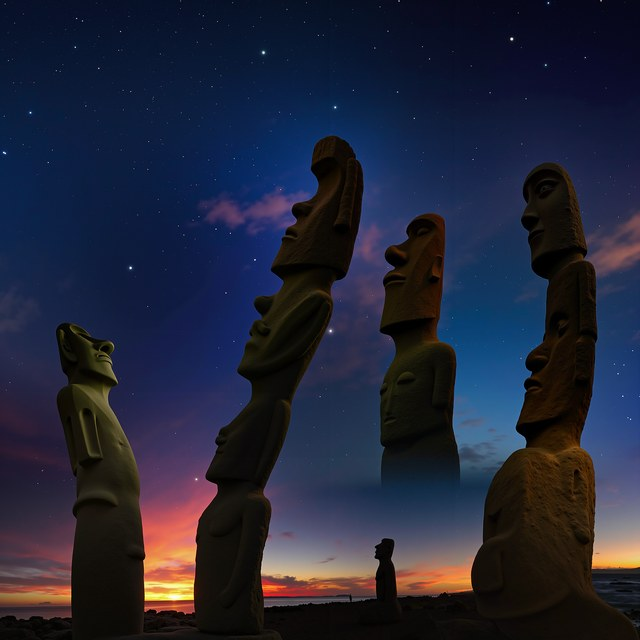
\includegraphics[height=0.1632\scaW]{figures/failures/dup_3614061571823823193_abl_v0.jpg}\hspace{0.0040\scaW}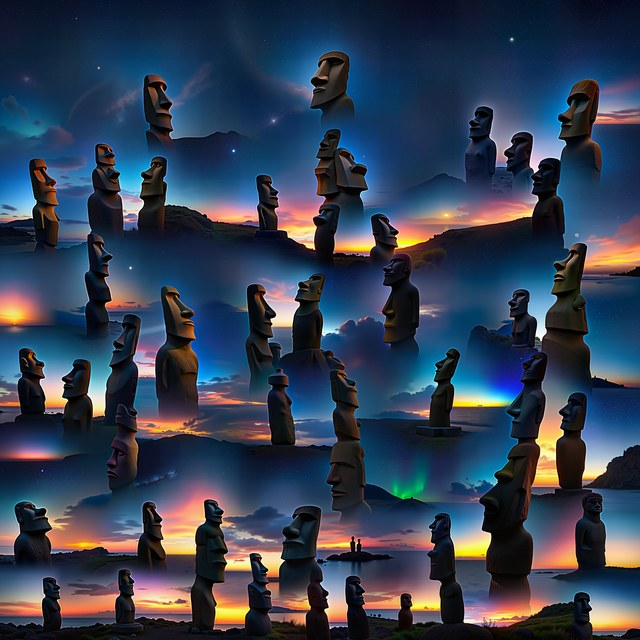
\includegraphics[height=0.1632\scaW]{figures/failures/dup_3614061571823823193_dev_w16.jpg}\hspace{0.0040\scaW}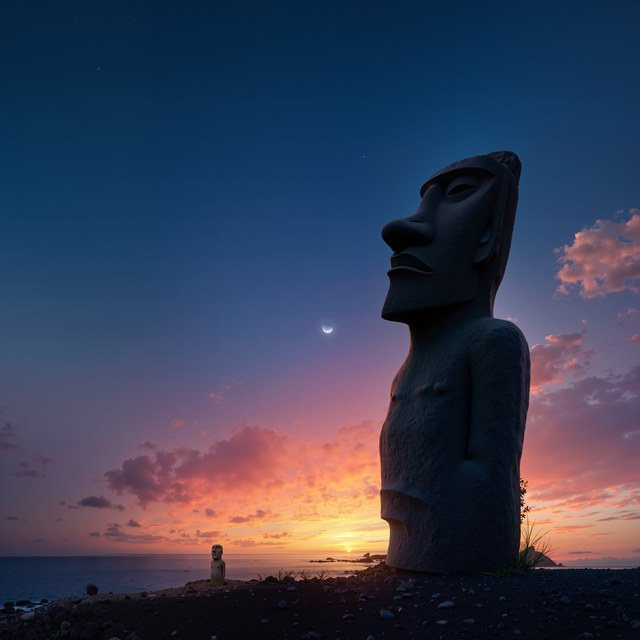
\includegraphics[height=0.1632\scaW]{figures/failures/dup_3614061571823823193_sca.jpg}}\\[0.0040\textwidth]
\makebox[\textwidth][l]{\makebox[0.1632\scaW][c]{SCA}\hspace{0.0040\scaW}\makebox[0.1632\scaW][c]{SCA crop}\hspace{0.0040\scaW}\makebox[0.1632\scaW][c]{AReA crop}\hspace{0.0040\scaW}\makebox[0.1632\scaW][c]{SCA}\hspace{0.0040\scaW}\makebox[0.1632\scaW][c]{SCA crop}\hspace{0.0040\scaW}\makebox[0.1632\scaW][c]{AReA crop}}\\[0.0040\textwidth]
\makebox[\textwidth][l]{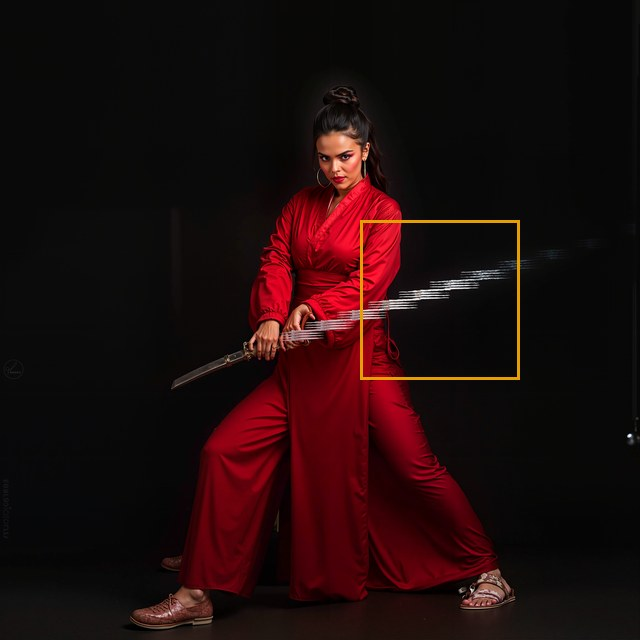
\includegraphics[height=0.1632\scaW]{figures/failures/err_7396058529551312081_sca.jpg}\hspace{0.0040\scaW}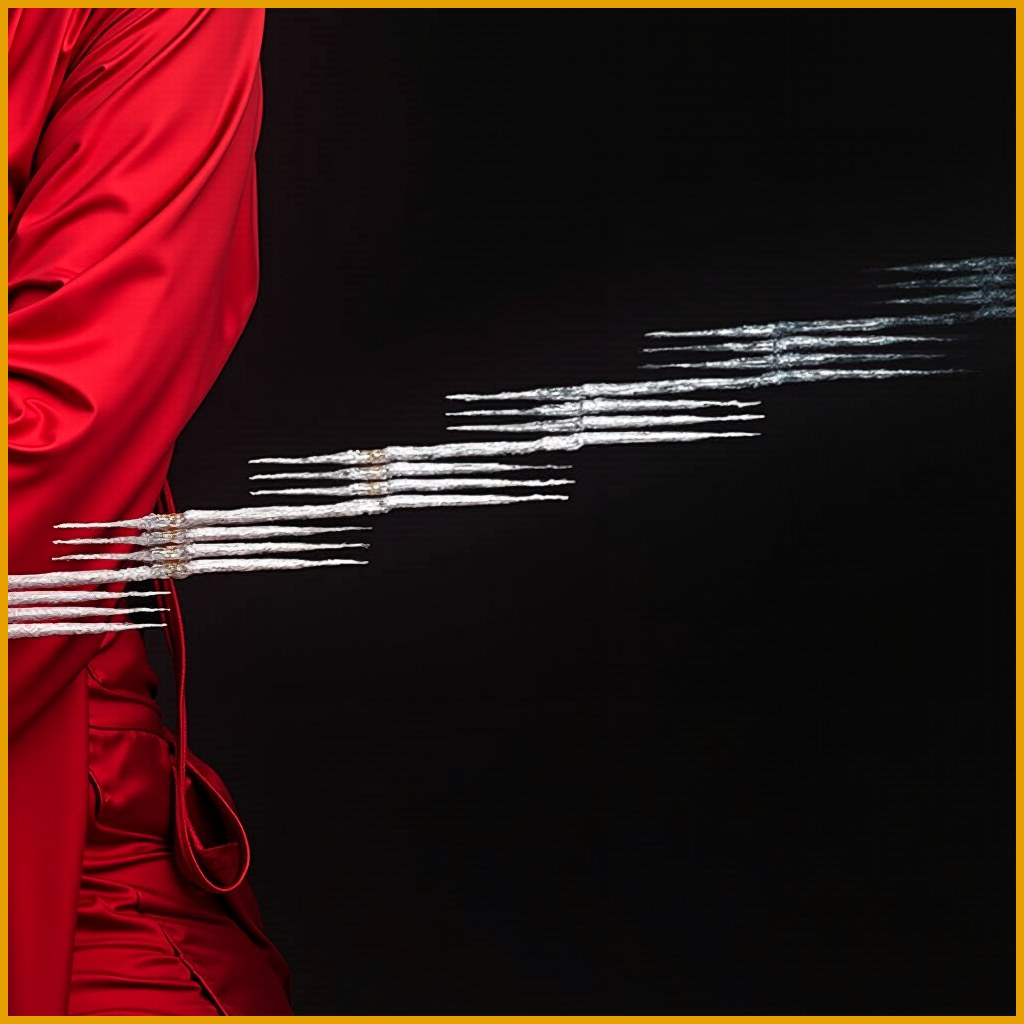
\includegraphics[height=0.1632\scaW]{figures/failures/err_7396058529551312081_sca_crop.jpg}\hspace{0.0040\scaW}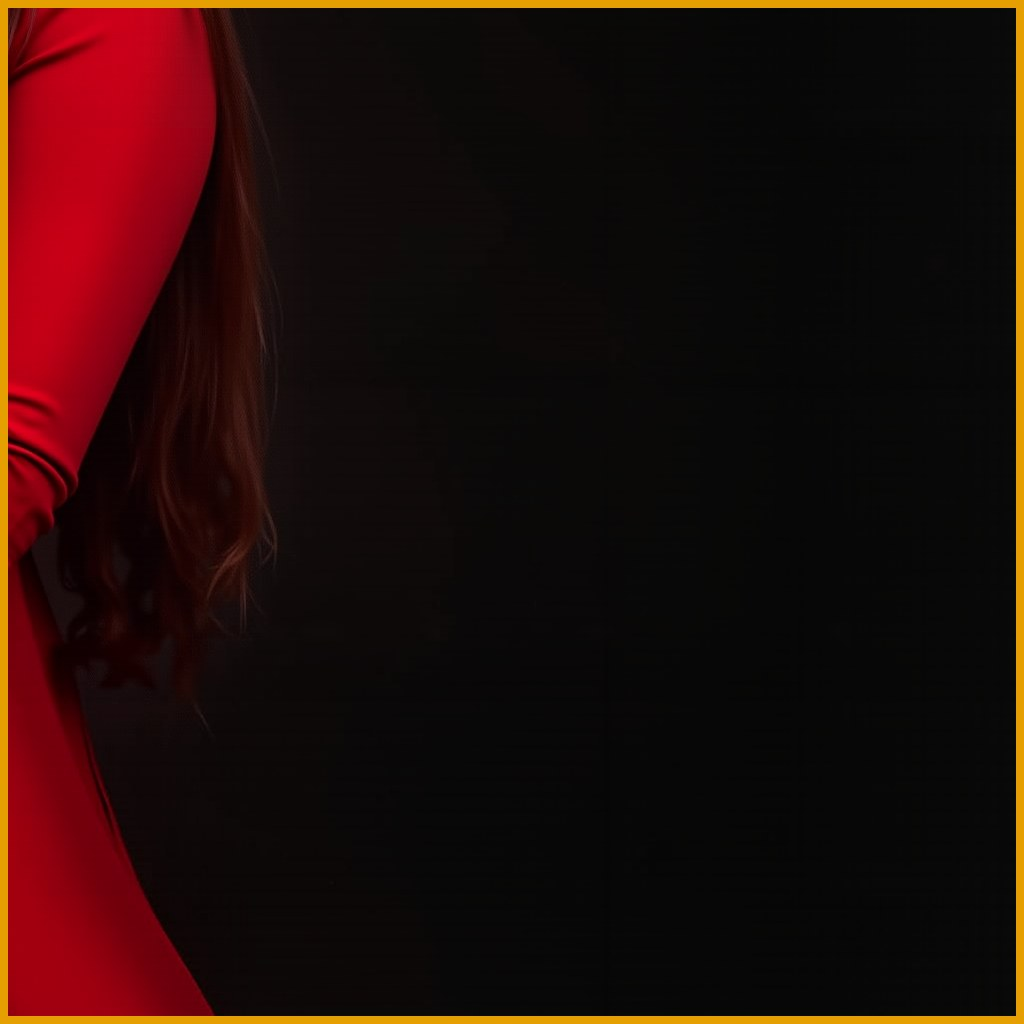
\includegraphics[height=0.1632\scaW]{figures/failures/err_7396058529551312081_area_crop.jpg}\hspace{0.0040\scaW}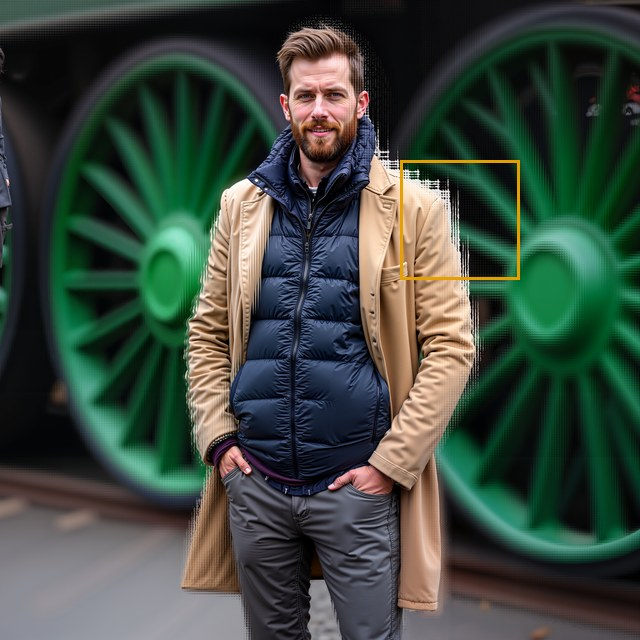
\includegraphics[height=0.1632\scaW]{figures/failures/err_1316997283360365550_sca.jpg}\hspace{0.0040\scaW}
\includegraphics[height=0.1632\scaW]{figures/failures/err_1316997283360365550_sca_crop.jpg}\hspace{0.0040\scaW}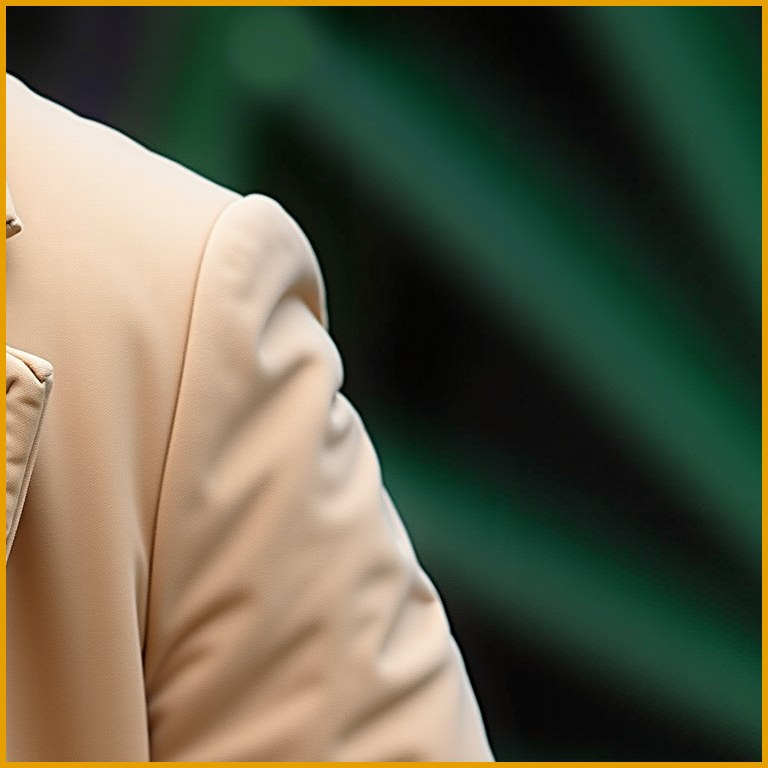
\includegraphics[height=0.1632\scaW]{figures/failures/err_1316997283360365550_area_crop.jpg}}\\[0.0040\textwidth]
\makebox[\textwidth][l]{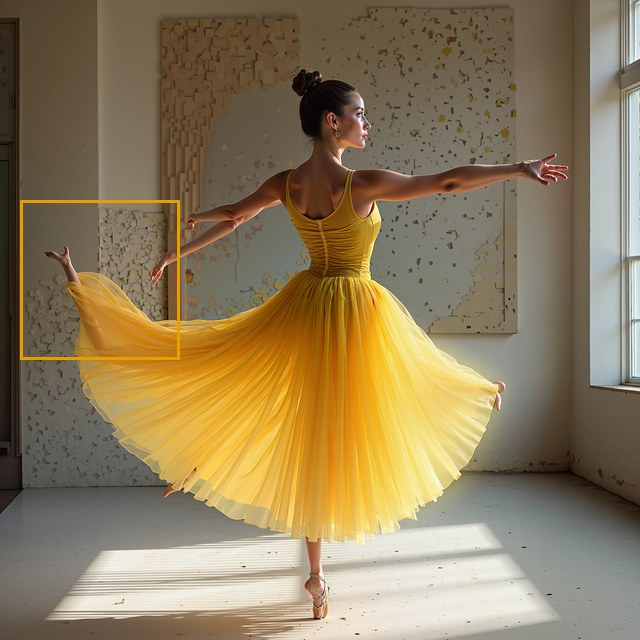
\includegraphics[height=0.1632\scaW]{figures/failures/err_m8648158440845565467_sca.jpg}\hspace{0.0040\scaW}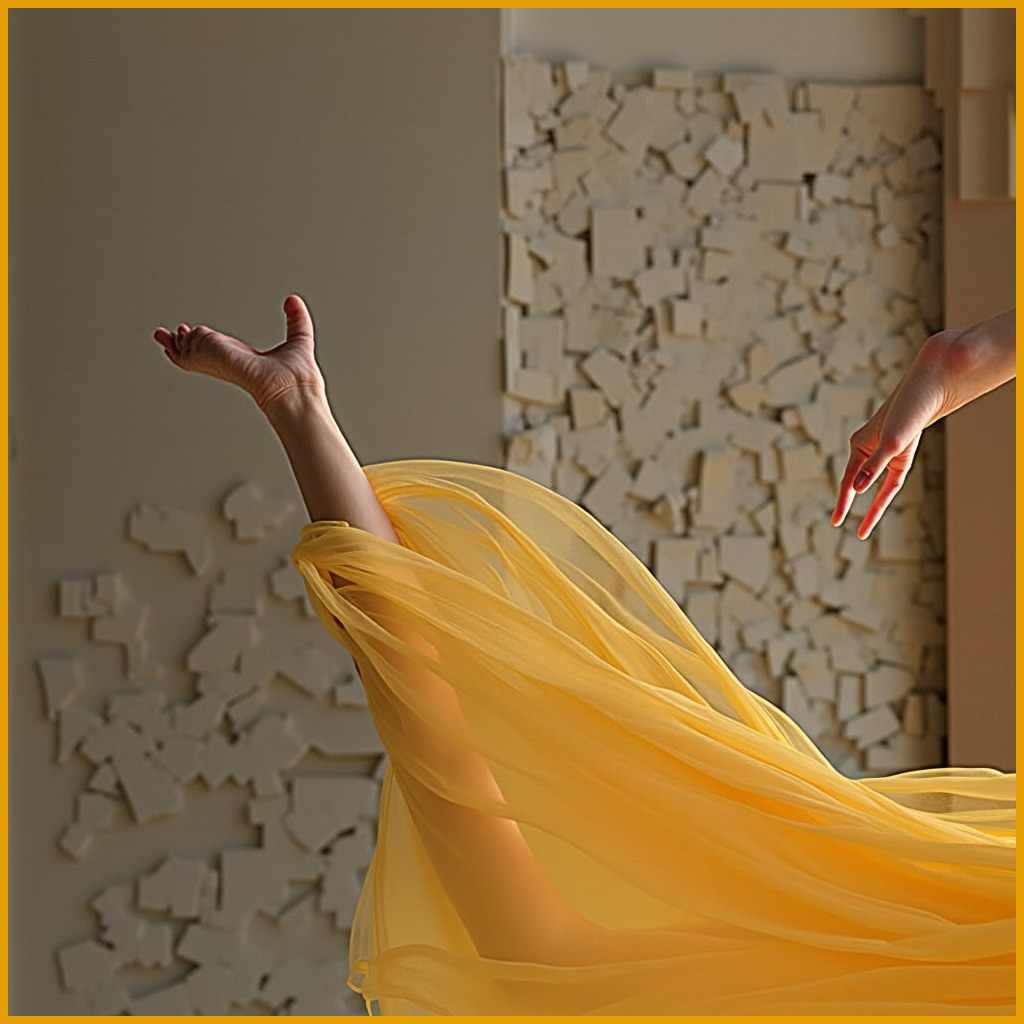
\includegraphics[height=0.1632\scaW]{figures/failures/err_m8648158440845565467_sca_crop.jpg}\hspace{0.0040\scaW}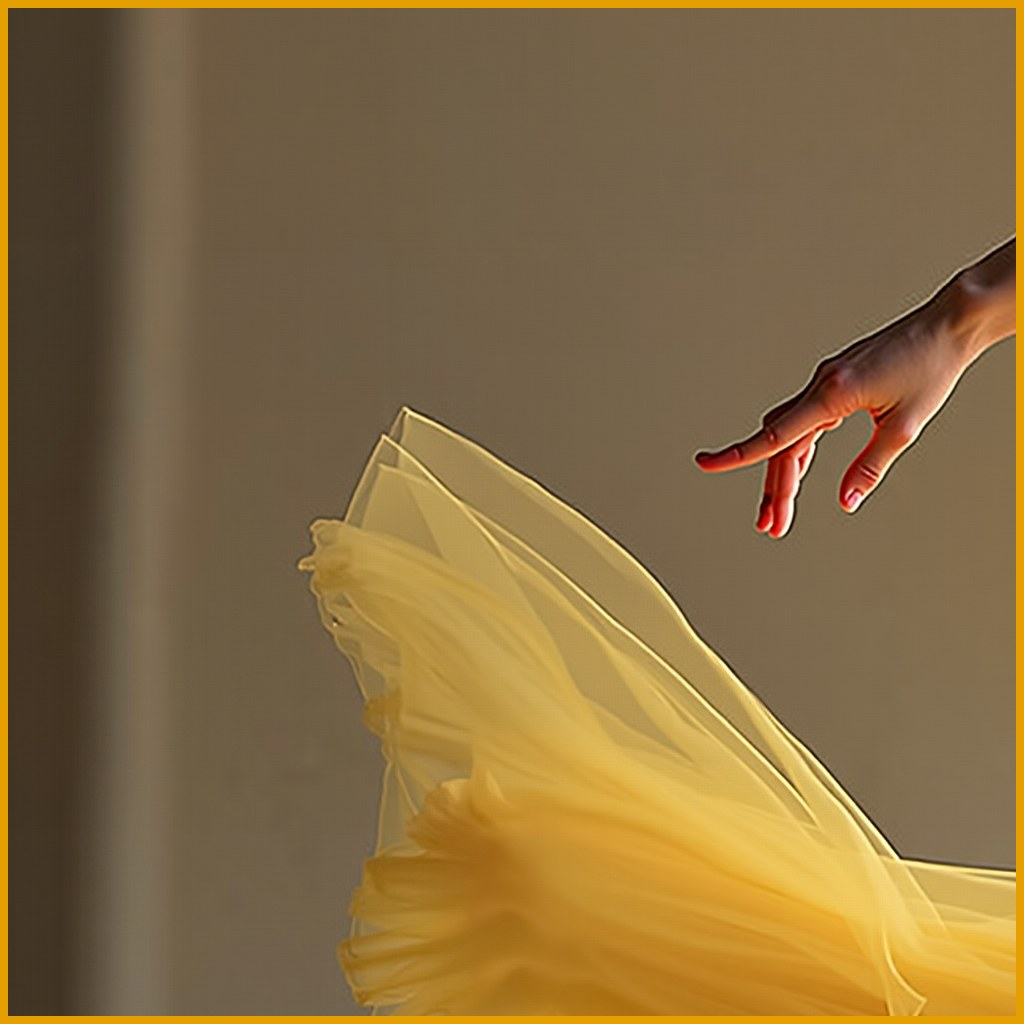
\includegraphics[height=0.1632\scaW]{figures/failures/err_m8648158440845565467_area_crop.jpg}\hspace{0.0040\scaW}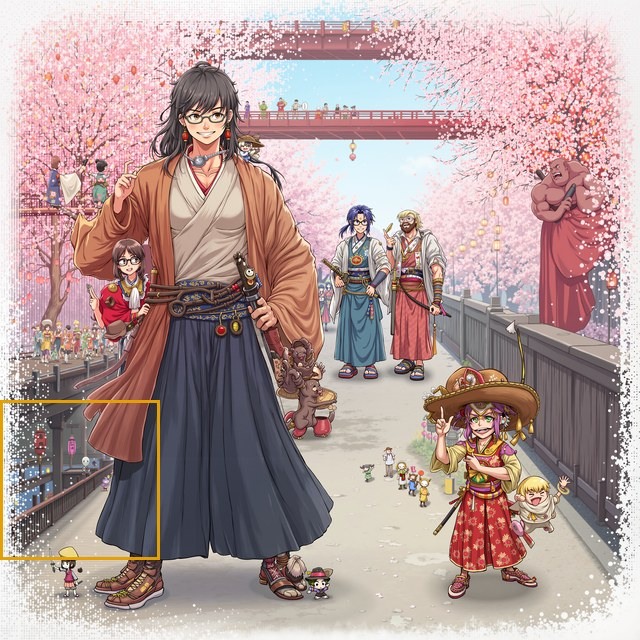
\includegraphics[height=0.1632\scaW]{figures/failures/err_m702025498990232048_sca.jpg}\hspace{0.0040\scaW}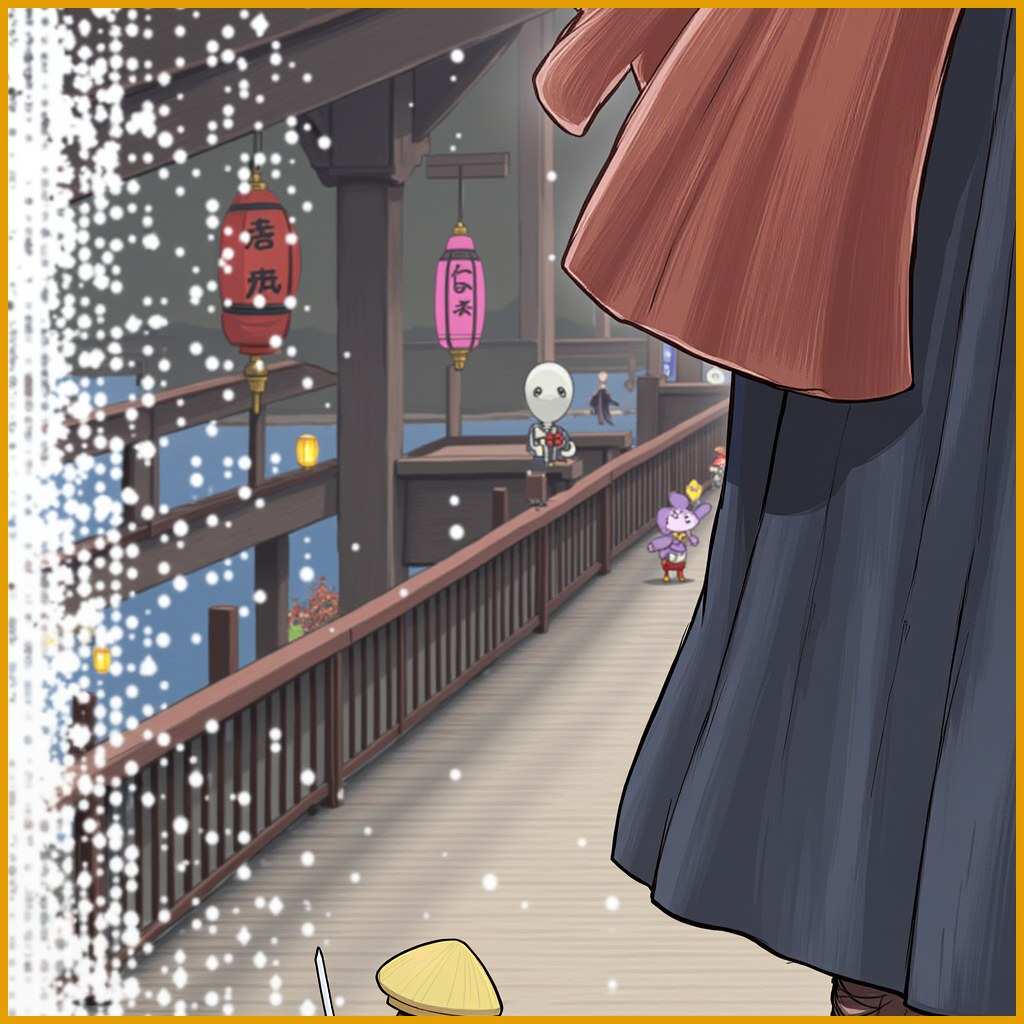
\includegraphics[height=0.1632\scaW]{figures/failures/err_m702025498990232048_sca_crop.jpg}\hspace{0.0040\scaW}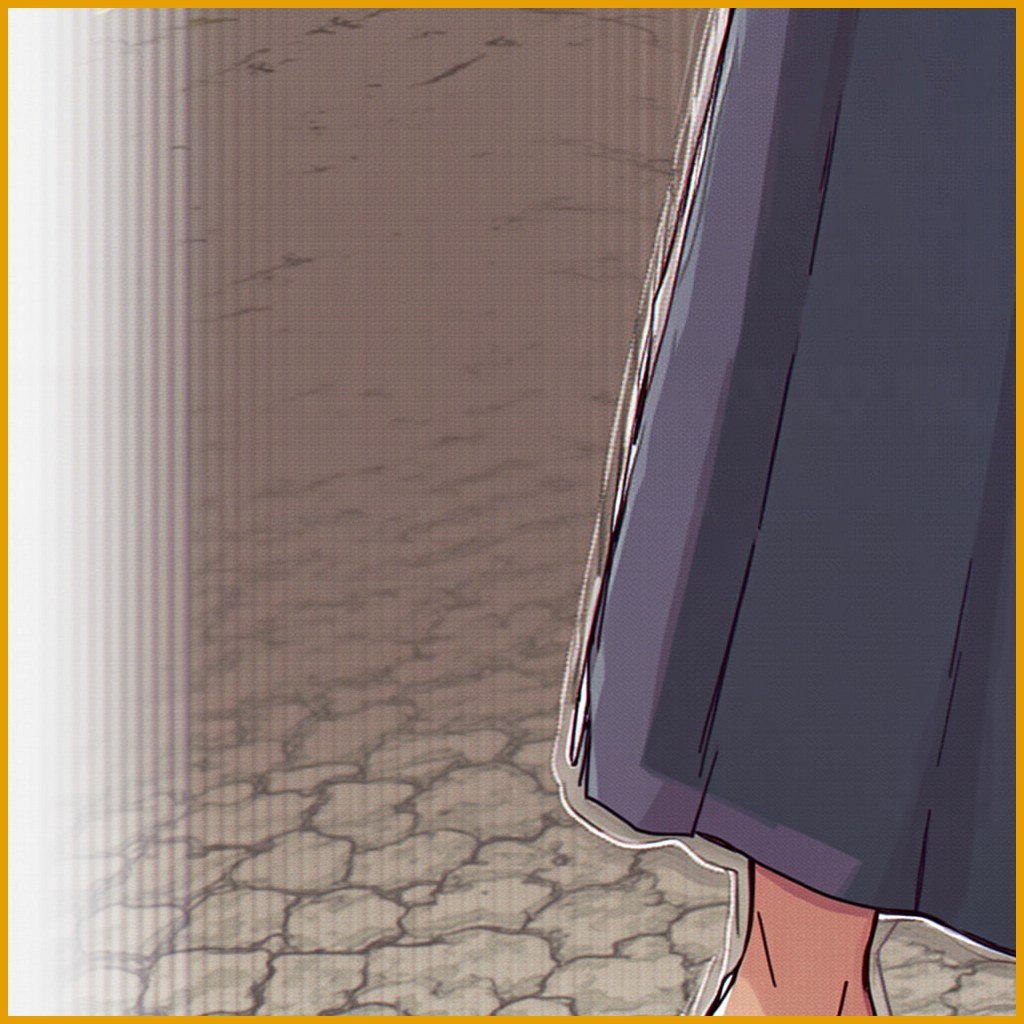
\includegraphics[height=0.1632\scaW]{figures/failures/err_m702025498990232048_area_crop.jpg}}
\rmfamily\normalsize
\caption{\textbf{Failure modes.} Top: without the gate, local windows decide the layout at high noise and duplicate the subject (no gate, 64-token window; no gate, 16-token window, which gives smaller and more numerous copies); SCA keeps one subject. Two development prompts, 4096$\times$4096. Middle and bottom: errors SCA still makes on evaluation prompts, with 1:1 crops of the outlined window and the same window from AReA. A thin diagonal sword is drawn as a staircase of short blocks; a patch beside the coat turns into a coarse grid; a dancer's rear arm ends in a foot; and the border of a dense illustration dissolves into speckle. AReA's images show none of these four errors, though its compositions differ, so its crops are not of the same objects. All seed 0.}
\label{fig:failures}
\end{figure*}

\clearpage
\noindent\texttt{snippet: gallery\_4096}\par% Generated by paper/figures/src/fig_qual.py gallery_4096; do not edit by hand.
% Rows split 2/12/2 by hand for the appendix page layout (prompt order unchanged; rerunning fig_qual.py gallery_4096 restores the 8/8 split and leaves a stale _p3).
% 1516768667427572324 (4096x4096): A cluttered artist's corner features an ornate gold frame, a painting of a man with glasses, several empty picture frames, a vintage suitcase, and var
% 2232973817337527860 (4096x4096): A bouquet of pink lilies is arranged in a clear vase filled with water, placed on a white side table next to a partially opened curtain and a closed d
% 3411143122470771726 (4096x4096): A muscular man with green hair and a sword stands confidently beside a woman in glasses and shorts, while a small animal in a red hat playfully trails
% 3638740675706761149 (4096x4096): Snow-capped mountains loom in the background, their peaks reflected in a calm lake surrounded by a rocky shore and green pine trees.
\input{figures/snippets/_scagrid}%
\begin{figure*}[!h]
\begingroup\scaGridStyle
\setlength{\scaT}{\dimexpr(\linewidth-21pt)*1000/8000\relax}%
\makebox[\linewidth][c]{\scaHead{\dimexpr2\scaT+1pt\relax}{scaMid}{AReA}\hspace{4pt}\scaHead{\dimexpr2\scaT+1pt\relax}{scaAccent}{\textcolor{scaAccent}{\textbf{SCA (ours)}}}\hspace{9pt}\scaHead{\dimexpr2\scaT+1pt\relax}{scaMid}{AReA}\hspace{4pt}\scaHead{\dimexpr2\scaT+1pt\relax}{scaAccent}{\textcolor{scaAccent}{\textbf{SCA (ours)}}}}\par\vskip2pt
\makebox[\linewidth][c]{\scaFull{\scaT}{\scaT}{figures/gallery_4096/1516768667427572324_area.jpg}{(0.64258,0.08008)}{(0.76758,0.20508)}\hspace{1pt}\scaCrop{\scaT}{\scaT}{figures/gallery_4096/1516768667427572324_area_crop.jpg}\hspace{4pt}\scaFull{\scaT}{\scaT}{figures/gallery_4096/1516768667427572324_sca.jpg}{(0.64258,0.08008)}{(0.76758,0.20508)}\hspace{1pt}\scaCrop{\scaT}{\scaT}{figures/gallery_4096/1516768667427572324_sca_crop.jpg}\hspace{9pt}\scaFull{\scaT}{\scaT}{figures/gallery_4096/2232973817337527860_area.jpg}{(0.32617,0.47852)}{(0.45117,0.60352)}\hspace{1pt}\scaCrop{\scaT}{\scaT}{figures/gallery_4096/2232973817337527860_area_crop.jpg}\hspace{4pt}\scaFull{\scaT}{\scaT}{figures/gallery_4096/2232973817337527860_sca.jpg}{(0.32617,0.47852)}{(0.45117,0.60352)}\hspace{1pt}\scaCrop{\scaT}{\scaT}{figures/gallery_4096/2232973817337527860_sca_crop.jpg}}\par\vskip2pt
\makebox[\linewidth][c]{\scaFull{\scaT}{\scaT}{figures/gallery_4096/3411143122470771726_area.jpg}{(0.39844,0.50195)}{(0.52344,0.62695)}\hspace{1pt}\scaCrop{\scaT}{\scaT}{figures/gallery_4096/3411143122470771726_area_crop.jpg}\hspace{4pt}\scaFull{\scaT}{\scaT}{figures/gallery_4096/3411143122470771726_sca.jpg}{(0.39844,0.50195)}{(0.52344,0.62695)}\hspace{1pt}\scaCrop{\scaT}{\scaT}{figures/gallery_4096/3411143122470771726_sca_crop.jpg}\hspace{9pt}\scaFull{\scaT}{\scaT}{figures/gallery_4096/3638740675706761149_area.jpg}{(0.06250,0.68945)}{(0.18750,0.81445)}\hspace{1pt}\scaCrop{\scaT}{\scaT}{figures/gallery_4096/3638740675706761149_area_crop.jpg}\hspace{4pt}\scaFull{\scaT}{\scaT}{figures/gallery_4096/3638740675706761149_sca.jpg}{(0.06250,0.68945)}{(0.18750,0.81445)}\hspace{1pt}\scaCrop{\scaT}{\scaT}{figures/gallery_4096/3638740675706761149_sca_crop.jpg}}\par
\endgroup
\caption{\textbf{Uncurated samples at 4096$\times$4096: AReA and \textbf{SCA (ours)}.} 32 evaluation prompts drawn at random (selection seed~0), excluding development and main-text prompts. FLUX.1-dev, seed~0, 28 steps, guidance 4.5. Each image is followed by a native-pixel crop of its outlined 512$\times$512 window of highest edge energy averaged over the methods.}
\label{fig:gallery_4096}
\end{figure*}

\clearpage
\noindent\texttt{snippet: gallery\_4096\_p2}\par% Generated by paper/figures/src/fig_qual.py gallery_4096; do not edit by hand.
% m1071233499893339092 (4096x4096): A solitary astronaut in a white spacesuit sits on a rock, surrounded by tall, rocky formations under a blue sky with soft clouds. The landscape is bar
% m2679953061215100202 (4096x4096): A dancer in mid-pose creates a dynamic splash of water, set against a black background, illuminated to highlight their silhouette.
% m2978915343052374306 (4096x4096): A man with long blonde hair, wearing a black leather jacket and a scarf, gazes down thoughtfully while holding a vintage Stratocaster guitar, featurin
% m3130703310573987496 (4096x4096): Rolling green hills under a clear blue sky, dotted with patches of mist and purple heather, feature a solitary tree and a weathered stone wall.
% m3514666929034129151 (4096x4096): A scuba diver hovers over rocky underwater terrain, with a clear blue sky and mountains visible above the water's surface.
% m4526778177368208567 (4096x4096): A young woman with long, straight white hair and captivating eyes turns her head profile, wearing a textured, oversized orange shirt. The background f
% m4844341235185759356 (4096x4096): A lone hiker stands on a rocky outcrop, overlooking a stunning landscape of dramatic mountains and a serene, reflective body of water at sunset, with 
% m493587068337986360 (4096x4096): A tranquil lake reflects colorful houses and a tall church steeple, surrounded by lush green mountains and a cloudy sky.
% m5606822722792416000 (4096x4096): A woman in a light blue dress stands at a balcony, holding onto the door frame, with a view of a serene coastal landscape featuring mountains and a pe
% m5673083787255800687 (4096x4096): A character in a vibrant red and patterned coat, holding a navy blue umbrella, stands gracefully among falling pink petals, with a decorative blue hat
% m5795767365495583614 (4096x4096): A large polar bear sits by a tranquil water's edge, reflecting the cloudy, moonlit sky, while a tiny figure stands on a rocky outcrop in the backgroun
% m653754125991313145 (4096x4096): A starry night sky filled with countless stars and the Milky Way stretches across the scene, highlighting rugged, eroded rock formations that rise dra
% m7169704122316291462 (4096x4096): A young man with an afro hairstyle wears reflective sunglasses and a fur-lined jacket, standing in front of vibrant neon signs in shades of pink and b
% m7321186811358178749 (4096x4096): Two dark ceramic plates feature thick slices of golden bread topped with green sauce, surrounded by white beans and fresh kale. A small bowl of green 
% m7459007800202269666 (4096x4096): A man and a woman stroll hand-in-hand down a narrow, cobblestone street, each holding a traditional parasol - one white and the other red - while wearing 
% m7946139341219184985 (4096x4096): Colorful historic buildings line a tranquil harbor, their reflections shimmering in the water, with several sailboats moored nearby and restaurants il
\input{figures/snippets/_scagrid}%
\begin{figure*}[t]
\begingroup\scaGridStyle
\setlength{\scaT}{\dimexpr(\linewidth-21pt)*1000/8000\relax}%
\makebox[\linewidth][c]{\scaHead{\dimexpr2\scaT+1pt\relax}{scaMid}{AReA}\hspace{4pt}\scaHead{\dimexpr2\scaT+1pt\relax}{scaAccent}{\textcolor{scaAccent}{\textbf{SCA (ours)}}}\hspace{9pt}\scaHead{\dimexpr2\scaT+1pt\relax}{scaMid}{AReA}\hspace{4pt}\scaHead{\dimexpr2\scaT+1pt\relax}{scaAccent}{\textcolor{scaAccent}{\textbf{SCA (ours)}}}}\par\vskip2pt
\makebox[\linewidth][c]{\scaFull{\scaT}{\scaT}{figures/gallery_4096/m1071233499893339092_area.jpg}{(0.42578,0.30859)}{(0.55078,0.43359)}\hspace{1pt}\scaCrop{\scaT}{\scaT}{figures/gallery_4096/m1071233499893339092_area_crop.jpg}\hspace{4pt}\scaFull{\scaT}{\scaT}{figures/gallery_4096/m1071233499893339092_sca.jpg}{(0.42578,0.30859)}{(0.55078,0.43359)}\hspace{1pt}\scaCrop{\scaT}{\scaT}{figures/gallery_4096/m1071233499893339092_sca_crop.jpg}\hspace{9pt}\scaFull{\scaT}{\scaT}{figures/gallery_4096/m2679953061215100202_area.jpg}{(0.31641,0.07812)}{(0.44141,0.20312)}\hspace{1pt}\scaCrop{\scaT}{\scaT}{figures/gallery_4096/m2679953061215100202_area_crop.jpg}\hspace{4pt}\scaFull{\scaT}{\scaT}{figures/gallery_4096/m2679953061215100202_sca.jpg}{(0.31641,0.07812)}{(0.44141,0.20312)}\hspace{1pt}\scaCrop{\scaT}{\scaT}{figures/gallery_4096/m2679953061215100202_sca_crop.jpg}}\par\vskip2pt
\makebox[\linewidth][c]{\scaFull{\scaT}{\scaT}{figures/gallery_4096/m2978915343052374306_area.jpg}{(0.34766,0.21289)}{(0.47266,0.33789)}\hspace{1pt}\scaCrop{\scaT}{\scaT}{figures/gallery_4096/m2978915343052374306_area_crop.jpg}\hspace{4pt}\scaFull{\scaT}{\scaT}{figures/gallery_4096/m2978915343052374306_sca.jpg}{(0.34766,0.21289)}{(0.47266,0.33789)}\hspace{1pt}\scaCrop{\scaT}{\scaT}{figures/gallery_4096/m2978915343052374306_sca_crop.jpg}\hspace{9pt}\scaFull{\scaT}{\scaT}{figures/gallery_4096/m3130703310573987496_area.jpg}{(0.22266,0.17773)}{(0.34766,0.30273)}\hspace{1pt}\scaCrop{\scaT}{\scaT}{figures/gallery_4096/m3130703310573987496_area_crop.jpg}\hspace{4pt}\scaFull{\scaT}{\scaT}{figures/gallery_4096/m3130703310573987496_sca.jpg}{(0.22266,0.17773)}{(0.34766,0.30273)}\hspace{1pt}\scaCrop{\scaT}{\scaT}{figures/gallery_4096/m3130703310573987496_sca_crop.jpg}}\par\vskip2pt
\makebox[\linewidth][c]{\scaFull{\scaT}{\scaT}{figures/gallery_4096/m3514666929034129151_area.jpg}{(0.06250,0.70117)}{(0.18750,0.82617)}\hspace{1pt}\scaCrop{\scaT}{\scaT}{figures/gallery_4096/m3514666929034129151_area_crop.jpg}\hspace{4pt}\scaFull{\scaT}{\scaT}{figures/gallery_4096/m3514666929034129151_sca.jpg}{(0.06250,0.70117)}{(0.18750,0.82617)}\hspace{1pt}\scaCrop{\scaT}{\scaT}{figures/gallery_4096/m3514666929034129151_sca_crop.jpg}\hspace{9pt}\scaFull{\scaT}{\scaT}{figures/gallery_4096/m4526778177368208567_area.jpg}{(0.25781,0.42578)}{(0.38281,0.55078)}\hspace{1pt}\scaCrop{\scaT}{\scaT}{figures/gallery_4096/m4526778177368208567_area_crop.jpg}\hspace{4pt}\scaFull{\scaT}{\scaT}{figures/gallery_4096/m4526778177368208567_sca.jpg}{(0.25781,0.42578)}{(0.38281,0.55078)}\hspace{1pt}\scaCrop{\scaT}{\scaT}{figures/gallery_4096/m4526778177368208567_sca_crop.jpg}}\par\vskip2pt
\makebox[\linewidth][c]{\scaFull{\scaT}{\scaT}{figures/gallery_4096/m4844341235185759356_area.jpg}{(0.42773,0.27344)}{(0.55273,0.39844)}\hspace{1pt}\scaCrop{\scaT}{\scaT}{figures/gallery_4096/m4844341235185759356_area_crop.jpg}\hspace{4pt}\scaFull{\scaT}{\scaT}{figures/gallery_4096/m4844341235185759356_sca.jpg}{(0.42773,0.27344)}{(0.55273,0.39844)}\hspace{1pt}\scaCrop{\scaT}{\scaT}{figures/gallery_4096/m4844341235185759356_sca_crop.jpg}\hspace{9pt}\scaFull{\scaT}{\scaT}{figures/gallery_4096/m493587068337986360_area.jpg}{(0.71680,0.40430)}{(0.84180,0.52930)}\hspace{1pt}\scaCrop{\scaT}{\scaT}{figures/gallery_4096/m493587068337986360_area_crop.jpg}\hspace{4pt}\scaFull{\scaT}{\scaT}{figures/gallery_4096/m493587068337986360_sca.jpg}{(0.71680,0.40430)}{(0.84180,0.52930)}\hspace{1pt}\scaCrop{\scaT}{\scaT}{figures/gallery_4096/m493587068337986360_sca_crop.jpg}}\par\vskip2pt
\makebox[\linewidth][c]{\scaFull{\scaT}{\scaT}{figures/gallery_4096/m5606822722792416000_area.jpg}{(0.12109,0.14844)}{(0.24609,0.27344)}\hspace{1pt}\scaCrop{\scaT}{\scaT}{figures/gallery_4096/m5606822722792416000_area_crop.jpg}\hspace{4pt}\scaFull{\scaT}{\scaT}{figures/gallery_4096/m5606822722792416000_sca.jpg}{(0.12109,0.14844)}{(0.24609,0.27344)}\hspace{1pt}\scaCrop{\scaT}{\scaT}{figures/gallery_4096/m5606822722792416000_sca_crop.jpg}\hspace{9pt}\scaFull{\scaT}{\scaT}{figures/gallery_4096/m5673083787255800687_area.jpg}{(0.80273,0.06250)}{(0.92773,0.18750)}\hspace{1pt}\scaCrop{\scaT}{\scaT}{figures/gallery_4096/m5673083787255800687_area_crop.jpg}\hspace{4pt}\scaFull{\scaT}{\scaT}{figures/gallery_4096/m5673083787255800687_sca.jpg}{(0.80273,0.06250)}{(0.92773,0.18750)}\hspace{1pt}\scaCrop{\scaT}{\scaT}{figures/gallery_4096/m5673083787255800687_sca_crop.jpg}}\par\vskip2pt
\makebox[\linewidth][c]{\scaFull{\scaT}{\scaT}{figures/gallery_4096/m5795767365495583614_area.jpg}{(0.78711,0.38281)}{(0.91211,0.50781)}\hspace{1pt}\scaCrop{\scaT}{\scaT}{figures/gallery_4096/m5795767365495583614_area_crop.jpg}\hspace{4pt}\scaFull{\scaT}{\scaT}{figures/gallery_4096/m5795767365495583614_sca.jpg}{(0.78711,0.38281)}{(0.91211,0.50781)}\hspace{1pt}\scaCrop{\scaT}{\scaT}{figures/gallery_4096/m5795767365495583614_sca_crop.jpg}\hspace{9pt}\scaFull{\scaT}{\scaT}{figures/gallery_4096/m653754125991313145_area.jpg}{(0.45898,0.57617)}{(0.58398,0.70117)}\hspace{1pt}\scaCrop{\scaT}{\scaT}{figures/gallery_4096/m653754125991313145_area_crop.jpg}\hspace{4pt}\scaFull{\scaT}{\scaT}{figures/gallery_4096/m653754125991313145_sca.jpg}{(0.45898,0.57617)}{(0.58398,0.70117)}\hspace{1pt}\scaCrop{\scaT}{\scaT}{figures/gallery_4096/m653754125991313145_sca_crop.jpg}}\par\vskip2pt
\makebox[\linewidth][c]{\scaFull{\scaT}{\scaT}{figures/gallery_4096/m7169704122316291462_area.jpg}{(0.69141,0.10547)}{(0.81641,0.23047)}\hspace{1pt}\scaCrop{\scaT}{\scaT}{figures/gallery_4096/m7169704122316291462_area_crop.jpg}\hspace{4pt}\scaFull{\scaT}{\scaT}{figures/gallery_4096/m7169704122316291462_sca.jpg}{(0.69141,0.10547)}{(0.81641,0.23047)}\hspace{1pt}\scaCrop{\scaT}{\scaT}{figures/gallery_4096/m7169704122316291462_sca_crop.jpg}\hspace{9pt}\scaFull{\scaT}{\scaT}{figures/gallery_4096/m7321186811358178749_area.jpg}{(0.43945,0.77148)}{(0.56445,0.89648)}\hspace{1pt}\scaCrop{\scaT}{\scaT}{figures/gallery_4096/m7321186811358178749_area_crop.jpg}\hspace{4pt}\scaFull{\scaT}{\scaT}{figures/gallery_4096/m7321186811358178749_sca.jpg}{(0.43945,0.77148)}{(0.56445,0.89648)}\hspace{1pt}\scaCrop{\scaT}{\scaT}{figures/gallery_4096/m7321186811358178749_sca_crop.jpg}}\par\vskip2pt
\makebox[\linewidth][c]{\scaFull{\scaT}{\scaT}{figures/gallery_4096/m7459007800202269666_area.jpg}{(0.25977,0.63867)}{(0.38477,0.76367)}\hspace{1pt}\scaCrop{\scaT}{\scaT}{figures/gallery_4096/m7459007800202269666_area_crop.jpg}\hspace{4pt}\scaFull{\scaT}{\scaT}{figures/gallery_4096/m7459007800202269666_sca.jpg}{(0.25977,0.63867)}{(0.38477,0.76367)}\hspace{1pt}\scaCrop{\scaT}{\scaT}{figures/gallery_4096/m7459007800202269666_sca_crop.jpg}\hspace{9pt}\scaFull{\scaT}{\scaT}{figures/gallery_4096/m7946139341219184985_area.jpg}{(0.20898,0.35742)}{(0.33398,0.48242)}\hspace{1pt}\scaCrop{\scaT}{\scaT}{figures/gallery_4096/m7946139341219184985_area_crop.jpg}\hspace{4pt}\scaFull{\scaT}{\scaT}{figures/gallery_4096/m7946139341219184985_sca.jpg}{(0.20898,0.35742)}{(0.33398,0.48242)}\hspace{1pt}\scaCrop{\scaT}{\scaT}{figures/gallery_4096/m7946139341219184985_sca_crop.jpg}}\par
\endgroup
\caption{\textbf{Uncurated samples at 4096$\times$4096: AReA and \textbf{SCA (ours)}, continued.} Same protocol as Figure~\ref{fig:gallery_4096}.}
\label{fig:gallery_4096_p2}
\end{figure*}

\clearpage
\noindent\texttt{snippet: gallery\_4096x2048}\par% Generated by paper/figures/src/fig_qual.py gallery_wide; do not edit by hand.
% 5898105534094229113 (2048x4096): A tranquil lake with smooth, dark rocks in the foreground reflects the deep blue sky and distant snow-capped mountains, as clouds streak across the ho
% 7637161027288029693 (2048x4096): A dramatic landscape features dark, swirling clouds above serene water, highlighted by rays of light breaking through. Several angular, purple-tinted 
% 9082507599514684465 (2048x4096): A young man in a white shirt and green tunic sits on a stone, using a measuring tool, while two standing figures, one in red robes with a turban and a
% m7320315357894569493.Jpg (2048x4096): A young man in a black ruffled outfit, adorned with a laurel crown, stands with his left hand resting on a pink pedestal, holding a book in his right 
% m836402013429605880 (2048x4096): A group of sheep stands in the snow, with a quaint stone church in the background, framed by trees adorned with snow. Two cozy houses peek through the
% m8573543815140502534 (2048x4096): A vast, starry night sky filled with the Milky Way illuminates surreal, eroded rock formations resembling hoodoos in a barren landscape.
\input{figures/snippets/_scagrid}%
\begin{figure*}[t]
\begingroup\scaGridStyle
\setlength{\scaT}{\dimexpr(\linewidth-6pt)*1000/6000\relax}%
\makebox[\linewidth][c]{\scaHead{\dimexpr3\scaT+1pt\relax}{scaMid}{AReA}\hspace{4pt}\scaHead{\dimexpr3\scaT+1pt\relax}{scaAccent}{\textcolor{scaAccent}{\textbf{SCA (ours)}}}}\par\vskip2pt
\makebox[\linewidth][c]{\scaFull{2\scaT}{\scaT}{figures/gallery_4096x2048/5898105534094229113_area.jpg}{(0.62500,0.47656)}{(0.75000,0.72656)}\hspace{1pt}\scaCrop{\scaT}{\scaT}{figures/gallery_4096x2048/5898105534094229113_area_crop.jpg}\hspace{4pt}\scaFull{2\scaT}{\scaT}{figures/gallery_4096x2048/5898105534094229113_sca.jpg}{(0.62500,0.47656)}{(0.75000,0.72656)}\hspace{1pt}\scaCrop{\scaT}{\scaT}{figures/gallery_4096x2048/5898105534094229113_sca_crop.jpg}}\par\vskip2pt
\makebox[\linewidth][c]{\scaFull{2\scaT}{\scaT}{figures/gallery_4096x2048/7637161027288029693_area.jpg}{(0.26367,0.25000)}{(0.38867,0.50000)}\hspace{1pt}\scaCrop{\scaT}{\scaT}{figures/gallery_4096x2048/7637161027288029693_area_crop.jpg}\hspace{4pt}\scaFull{2\scaT}{\scaT}{figures/gallery_4096x2048/7637161027288029693_sca.jpg}{(0.26367,0.25000)}{(0.38867,0.50000)}\hspace{1pt}\scaCrop{\scaT}{\scaT}{figures/gallery_4096x2048/7637161027288029693_sca_crop.jpg}}\par\vskip2pt
\makebox[\linewidth][c]{\scaFull{2\scaT}{\scaT}{figures/gallery_4096x2048/9082507599514684465_area.jpg}{(0.75195,0.47656)}{(0.87695,0.72656)}\hspace{1pt}\scaCrop{\scaT}{\scaT}{figures/gallery_4096x2048/9082507599514684465_area_crop.jpg}\hspace{4pt}\scaFull{2\scaT}{\scaT}{figures/gallery_4096x2048/9082507599514684465_sca.jpg}{(0.75195,0.47656)}{(0.87695,0.72656)}\hspace{1pt}\scaCrop{\scaT}{\scaT}{figures/gallery_4096x2048/9082507599514684465_sca_crop.jpg}}\par\vskip2pt
\makebox[\linewidth][c]{\scaFull{2\scaT}{\scaT}{figures/gallery_4096x2048/m7320315357894569493.Jpg_area.jpg}{(0.17969,0.06250)}{(0.30469,0.31250)}\hspace{1pt}\scaCrop{\scaT}{\scaT}{figures/gallery_4096x2048/m7320315357894569493.Jpg_area_crop.jpg}\hspace{4pt}\scaFull{2\scaT}{\scaT}{figures/gallery_4096x2048/m7320315357894569493.Jpg_sca.jpg}{(0.17969,0.06250)}{(0.30469,0.31250)}\hspace{1pt}\scaCrop{\scaT}{\scaT}{figures/gallery_4096x2048/m7320315357894569493.Jpg_sca_crop.jpg}}\par\vskip2pt
\makebox[\linewidth][c]{\scaFull{2\scaT}{\scaT}{figures/gallery_4096x2048/m836402013429605880_area.jpg}{(0.79883,0.68750)}{(0.92383,0.93750)}\hspace{1pt}\scaCrop{\scaT}{\scaT}{figures/gallery_4096x2048/m836402013429605880_area_crop.jpg}\hspace{4pt}\scaFull{2\scaT}{\scaT}{figures/gallery_4096x2048/m836402013429605880_sca.jpg}{(0.79883,0.68750)}{(0.92383,0.93750)}\hspace{1pt}\scaCrop{\scaT}{\scaT}{figures/gallery_4096x2048/m836402013429605880_sca_crop.jpg}}\par\vskip2pt
\makebox[\linewidth][c]{\scaFull{2\scaT}{\scaT}{figures/gallery_4096x2048/m8573543815140502534_area.jpg}{(0.57812,0.35547)}{(0.70312,0.60547)}\hspace{1pt}\scaCrop{\scaT}{\scaT}{figures/gallery_4096x2048/m8573543815140502534_area_crop.jpg}\hspace{4pt}\scaFull{2\scaT}{\scaT}{figures/gallery_4096x2048/m8573543815140502534_sca.jpg}{(0.57812,0.35547)}{(0.70312,0.60547)}\hspace{1pt}\scaCrop{\scaT}{\scaT}{figures/gallery_4096x2048/m8573543815140502534_sca_crop.jpg}}\par
\endgroup
\caption{\textbf{Uncurated samples at 4096$\times$2048 (width$\times$height): AReA and \textbf{SCA (ours)}.} Six evaluation prompts drawn at random, disjoint from the other galleries, excluding development and main-text prompts. FLUX.1-dev, seed~0, 28 steps, guidance 4.5. Each image is followed by a native-pixel crop of its outlined 512$\times$512 window of highest edge energy averaged over the methods.}
\label{fig:gallery_4096x2048}
\end{figure*}

\clearpage
\noindent\texttt{snippet: gallery\_6144x2048}\par% Generated by paper/figures/src/fig_gallery_large.py; do not edit by hand.
% Shows the first 2 of the 6 prompts in the frozen draw order of gallery_6144x2048/provenance.json (see its display record), in draw order.
% fig_qual.py and fig_phase2.py skip this gallery while its provenance.json has a display record.
% 7202527118696509246 (2048x6144): A climber in a red jacket and headlamp navigates a snowy mountain ridge at dusk, surrounded by jagged peaks and clouds.
% 8899498425633254014 (2048x6144): A solitary tree stands on rocky terrain under a dramatic sky, with vibrant sunset hues orange and yellow illuminating the landscape.
\input{figures/snippets/_scagrid}%
\begin{figure*}[t]
\begingroup\scaGridStyle
\setlength{\scaT}{\dimexpr(\linewidth-1pt-\scaLW-\scaLG)*1000/4000\relax}%
\makebox[\linewidth][c]{\hspace*{\dimexpr\scaLW+\scaLG\relax}\scaHead{3\scaT}{scaMid}{Full image}\hspace{1pt}\scaHead{\scaT}{scaMid}{1:1 crop}}\par\vskip2pt
\makebox[\linewidth][c]{\scaRowLabel{\scaT}{AReA}\hspace{\scaLG}\scaFull{3\scaT}{\scaT}{figures/gallery_6144x2048/7202527118696509246_area.jpg}{(0.59896,0.22656)}{(0.68229,0.47656)}\hspace{1pt}\scaCrop{\scaT}{\scaT}{figures/gallery_6144x2048/7202527118696509246_area_crop.jpg}}\par\vskip1pt
\makebox[\linewidth][c]{\scaRowLabel{\scaT}{\textcolor{scaAccent}{\textbf{SCA (ours)}}}\hspace{\scaLG}\scaFull{3\scaT}{\scaT}{figures/gallery_6144x2048/7202527118696509246_sca.jpg}{(0.59896,0.22656)}{(0.68229,0.47656)}\hspace{1pt}\scaCrop{\scaT}{\scaT}{figures/gallery_6144x2048/7202527118696509246_sca_crop.jpg}}\par\vskip5pt
\makebox[\linewidth][c]{\scaRowLabel{\scaT}{AReA}\hspace{\scaLG}\scaFull{3\scaT}{\scaT}{figures/gallery_6144x2048/8899498425633254014_area.jpg}{(0.32552,0.31250)}{(0.40885,0.56250)}\hspace{1pt}\scaCrop{\scaT}{\scaT}{figures/gallery_6144x2048/8899498425633254014_area_crop.jpg}}\par\vskip1pt
\makebox[\linewidth][c]{\scaRowLabel{\scaT}{\textcolor{scaAccent}{\textbf{SCA (ours)}}}\hspace{\scaLG}\scaFull{3\scaT}{\scaT}{figures/gallery_6144x2048/8899498425633254014_sca.jpg}{(0.32552,0.31250)}{(0.40885,0.56250)}\hspace{1pt}\scaCrop{\scaT}{\scaT}{figures/gallery_6144x2048/8899498425633254014_sca_crop.jpg}}\par
\endgroup
\caption{\textbf{Uncurated samples at 2048$\times$6144 (height$\times$width): AReA and \textbf{SCA (ours)}.} The first two of six evaluation prompts drawn at random, disjoint from the other galleries, excluding development and main-text prompts. FLUX.1-dev, seed~0, 28 steps, guidance 4.5. Crops are native-pixel views of the outlined 512$\times$512 window of highest edge energy averaged over the methods.}
\label{fig:gallery_6144x2048}
\end{figure*}

\clearpage
\noindent\texttt{snippet: hero}\par% Generated by src/fig_showcase.py (TikZ source src/showcase.tex, assets figures/showcase/);
% edit the script, not this file. Curated SCA outputs, seed 0; sources (role, prompt id, HxW):
% panorama: Great Wall 4230887929316158402 (2048x6144): A snowy ridge of the Great Wall of China stretches along a rugged mountain peak, illuminated by the golden light of dawn, above a sea of clo
% square: portrait minus1066207185399086750 (4096x4096): A woman with styled hair wears elegant glasses and multiple pieces of silver jewelry, including dangling earrings and layered necklaces, aga
% square: woman with owl minus7264311869050248176 (4096x4096): A woman in a black dress with intricate lace detailing stands in a forest, gazing over her shoulder at a large owl with outstretched wings, 
% square: still life minus8919475713516982506 (4096x4096): A decorative vase with floral branches and white blossoms sits on a light cloth, accompanied by a shiny red apple.
% square: ice climber 997293625843621481 (4096x4096): A climber, wearing a helmet and blue clothing, ascends through a narrow, icy crevice, using an ice axe for support amidst glacial blue ice f
% wide: dancer underwater minus9196631274539277035 (2048x4096): A woman in a flowing red dress dances gracefully underwater, with her long hair swirling around her, against a backdrop of clear blue water 
% wide: river town minus5370774387421928008 (2048x4096): A picturesque riverside scene featuring a medieval castle atop a hill, surrounded by vibrant autumn foliage, with colorful homes lining the 
\begin{figure*}[!ht]
  \centering
  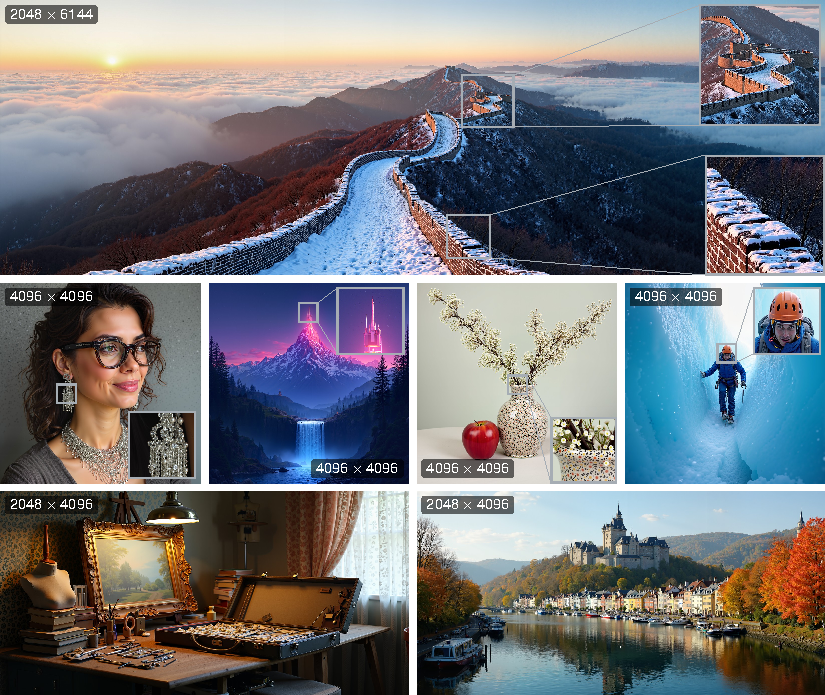
\includegraphics[width=\linewidth]{figures/showcase.pdf}
  \caption{\textbf{\sca{} keeps layout and fine detail across three aspect ratios without training.} Curated \sca{} outputs at $4096^2$, $2048\times4096$ and $2048\times6144$, picked by eye for clean results, so curation favours \sca{}; insets are 1:1 crops.}
  \label{fig:hero}
\end{figure*}

\clearpage
\noindent\texttt{snippet: latency}\par% Generated by paper/figures/src/fig_latency.py from results/latency_curve.csv.
\begin{figure}[t]
  \centering
  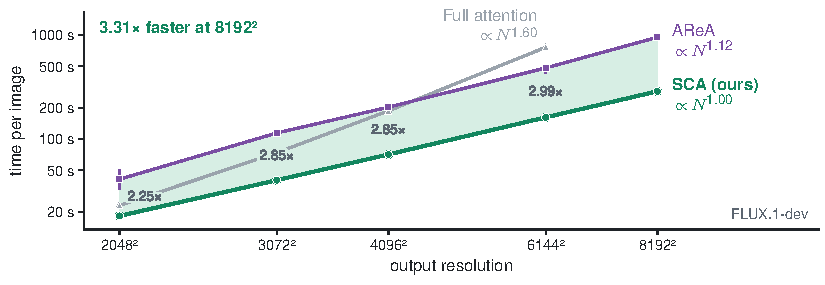
\includegraphics{figures/latency.pdf}
  \caption{\textbf{Measured generation latency across resolutions.}
  Seconds per image at batch size 1 on an idle GH200, including text encoding and VAE decoding. Points are medians of three prompts after a generated warm-up; whiskers show the observed minimum and maximum, not confidence intervals. The continuing sweep currently reaches $8192^2$ for SCA and $4096^2$ for both baselines. At $4096^2$, SCA takes 71.1\,s, full attention 186.5\,s, and AReA 202.4\,s.}
  \label{fig:latency}
\end{figure}

\clearpage
\noindent\texttt{snippet: method}\par% Method figure. Source: figures/src/method.tex (self-contained TikZ; build with `tectonic --outdir .. method.tex` in figures/src).
\begin{figure*}[t]
  \centering
  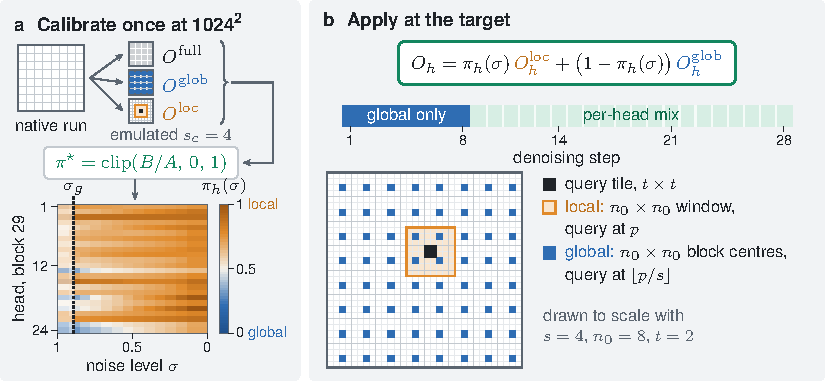
\includegraphics[width=\linewidth]{figures/method.pdf}
  \caption{\textbf{\sca{} mixes a native-size local window with block-centre global keys.} The opening steps, $\sigma>\sigma_g$, use the global operator alone, since high-noise windows repeat structure. Afterwards each head weights the local output by $\pi$, fitted once at $1024^2$ by matching full attention (right: one block's 24 heads by 14 noise bins).}
  \label{fig:method}
\end{figure*}

\clearpage
\noindent\texttt{snippet: qual\_main}\par% Generated by src/fig_qual_main.py (TikZ source src/qual_main.tex, assets figures/qual_main/cmp_*).
\begin{figure}[t]
  \centering
  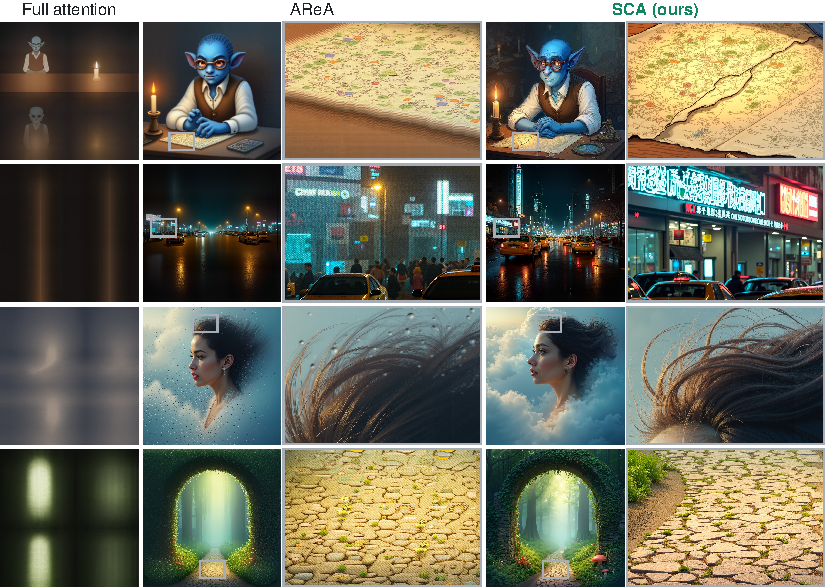
\includegraphics[width=\linewidth]{figures/qual_main.pdf}
  \caption{\textbf{At $4096^2$ full attention collapses, AReA blurs or tiles fine structure, and \sca{} keeps both layout and detail.} Four evaluation prompts, seed 0; next to each image is the same native $512\times512$ window, placed automatically where the three methods have the most edge energy. Random uncurated samples are in Figure~\ref{fig:gallery_4096}.}
  \label{fig:qual_main}
\end{figure}

\clearpage
\end{document}
